\documentclass[11pt]{article}
\usepackage[margin=1in]{geometry}
\usepackage{amsmath,graphicx,booktabs,hyperref}
\sloppy
% generated by scripts/tools/flight_design.py - do not edit
\newcommand{\flDuckModelG}{737}
\newcommand{\flDuckG}{812}
\newcommand{\flAllUpG}{1627}
\newcommand{\flThrustG}{2506}
\newcommand{\flTW}{1.54}
\newcommand{\flHoverPct}{65}
\newcommand{\flHoverW}{981}
\newcommand{\flHoverA}{71}
\newcommand{\flHoverS}{49}
\newcommand{\flMaxA}{158}
\newcommand{\flXc}{-13.1}
\newcommand{\flComX}{-13.1}
\newcommand{\flComZ}{168}
\newcommand{\flIxx}{17.4}
\newcommand{\flIyy}{9.9}
\newcommand{\flIzz}{12.0}
\newcommand{\flAccRoll}{67}
\newcommand{\flAccPitch}{36}
\newcommand{\flAccYaw}{11}
\newcommand{\flTauRoll}{1.16}
\newcommand{\flTauPitch}{0.36}
\newcommand{\flTauYaw}{0.127}
\newcommand{\flClrStand}{39}
\newcommand{\flHeadClr}{62}
\newcommand{\flSitPct}{23}
\newcommand{\flFoldPct}{21}
\newcommand{\flSitDx}{+10.4}
\newcommand{\flFoldDx}{-9.7}
\newcommand{\flArmL}{73}
\newcommand{\flArmI}{2456}
\newcommand{\flArmSigABS}{3.4}
\newcommand{\flArmSFABS}{12}
\newcommand{\flArmSFPLA}{16}
\newcommand{\flArmDeflABS}{0.57}
\newcommand{\flArmDeflPLA}{0.38}
\newcommand{\flArmHzABS}{70}
\newcommand{\flArmHzPLA}{86}
\newcommand{\flOpenRatioPct}{79}
\newcommand{\flTwLow}{1.17}
\newcommand{\flTwHigh}{2.00}
\newcommand{\flTwoFanTW}{1.13}
\newcommand{\flTwoFanBigTW}{1.48}
\newcommand{\flHoverWOpt}{715}
\newcommand{\flHoverSOpt}{70}
\newcommand{\flTetherG}{1464}
\newcommand{\flTetherTW}{1.97}
\newcommand{\flTetherA}{58}
\newcommand{\flTetherW}{844}
\newcommand{\flRollWorstDeg}{+22}
\newcommand{\flRollWorstY}{97}
\newcommand{\flRollClearLo}{-22}
\newcommand{\flRollClearHi}{+22}
\newcommand{\flBattAh}{1.3}
\newcommand{\flBattG}{163}
\newcommand{\flMaxC}{121}
\newcommand{\flHoverC}{55}
\newcommand{\flFrameG}{273}
\newcommand{\flFrameSrc}{CAD}

% generated by scripts/tools/flight_power.py
\newcommand{\fpPackMah}{1300}
\newcommand{\fpPackG}{163}
\newcommand{\fpPackTW}{1.67}
\newcommand{\fpPackVfull}{11.7}
\newcommand{\fpPackHoverA}{62}
\newcommand{\fpPackHoverW}{871}
\newcommand{\fpPackC}{48}
\newcommand{\fpPackDT}{16}
\newcommand{\fpPackSoc}{40}
\newcommand{\fpPackHoverS}{56}
\newcommand{\fpPackAllUp}{1497}
\newcommand{\fpFanKf}{2.04}
\newcommand{\fpFanKq}{2.34}
\newcommand{\fpFanEta}{0.51}
\newcommand{\fpPackUhover}{63}

% generated by scripts/tools/flight_report.py
\newcommand{\frStDefl}{1.8}
\newcommand{\frStTilt}{1.1}
\newcommand{\frStVm}{4.9}
\newcommand{\frStSfMin}{3.3}
\newcommand{\frStSfMinB}{3.4}
\newcommand{\frStWorst}{handling 20 N}
\newcommand{\frStMode}{25}
\newcommand{\frStModeB}{27}
\newcommand{\frStDofs}{316}
\newcommand{\frStMesh}{4}
\newcommand{\frStConvMesh}{3}
\newcommand{\frStConvDofs}{502}
\newcommand{\frStConvDefl}{-17}
\newcommand{\frStConvVm}{-18}
\newcommand{\frStConvMode}{27}
\newcommand{\frStCoreE}{74}
\newcommand{\frStCoreS}{0.87}
\newcommand{\frStFeMass}{204}
\newcommand{\frFrameABS}{232}
\newcommand{\frFramePLA}{273}
\newcommand{\frFramePLAB}{300}
\newcommand{\frSpanY}{331}
\newcommand{\frLenX}{145}
\newcommand{\frNParts}{11}
\newcommand{\frClrHead}{17.6}
\newcommand{\frClrLeg}{23.7}
\newcommand{\frClrHeadOld}{61.8}
\newcommand{\frClrLegOld}{18.9}
\newcommand{\frToolNeed}{28}
\newcommand{\frToolMin}{48}
\newcommand{\frToolN}{8}
\newcommand{\frToolOk}{8}
\newcommand{\frRobAssist}{0.8}
\newcommand{\frSidKfErr}{+0.2}
\newcommand{\frSidKfPrior}{-11}
\newcommand{\frSidRErr}{+19}
\newcommand{\frSidJErr}{-1.5}
\newcommand{\frSidDelayErr}{-0.9}
\newcommand{\frSidRzeroErr}{+0.1}
\newcommand{\frSidHoverPrior}{102.1}
\newcommand{\frSidHoverFit}{99.7}
\newcommand{\frCarryWalkBare}{0.39}
\newcommand{\frCarryRunBare}{0.58}
\newcommand{\frCarryWalkFalls}{6/6}
\newcommand{\frCarryRunFalls}{6/6}
\newcommand{\frRoRun}{0.40}
\newcommand{\frRoVlift}{0.56}
\newcommand{\frRoTilt}{33}
\newcommand{\frRoZerr}{13}
\newcommand{\frRoHoverV}{7}
\newcommand{\frRoU}{64}
\newcommand{\frRoI}{69}
\newcommand{\frRoV}{14.5}
\newcommand{\frRoSoc}{15}
\newcommand{\frRoX}{1.4}
\newcommand{\frRobOk}{20}
\newcommand{\frRobN}{25}
\newcommand{\frRobThrustOk}{5/5}
\newcommand{\frRobComSmallOk}{8/10}
\newcommand{\frRobComBigOk}{7/10}
\newcommand{\frRlSteps}{2.3}
\newcommand{\frRlMin}{68}
\newcommand{\frRlBaseOk}{31}
\newcommand{\frRlPolOk}{38}
\newcommand{\frRlBaseVxy}{0.25}
\newcommand{\frRlPolVxy}{0.59}
\newcommand{\frRlBaseVz}{0.20}
\newcommand{\frRlPolVz}{0.15}
\newcommand{\frRlLegDeg}{13}
\newcommand{\frRlGridBase}{11}
\newcommand{\frRlGridPol}{10}
\newcommand{\frRlNomVxy}{0.45}
\newcommand{\frRlNomVz}{0.15}
\newcommand{\frRlNomTilt}{11}
\newcommand{\frPackG}{815}

\makeatletter\let\tabinput\@@input\makeatother

\title{A Flying MicroDuck: Ducted-Fan Sizing, Fan and Pack Model, Identification, a Printed Wing Frame, and Run-to-Take-off Control}
\author{MicroDuck replication (Feetech HD1910 build)}
\date{2026-11-27 \quad design and simulation; nothing built, identified on hardware, or trained yet}

\begin{document}
\maketitle

\begin{abstract}
We design a ducted-fan pack that lets the 25\,cm MicroDuck biped run, take off, hover and land. Four
50\,mm fans on one 4S pack are sized with a grey-box model of the fan, ESC and battery that includes
voltage sag: catalogue thrust is quoted near 16\,V, but four fans pull the pack to
\fpPackVfull\,V, which changes the fan choice (5000\,KV, thrust-to-weight \fpPackTW) and fixes the
smallest pack (4S \fpPackMah\,mAh, \fpPackG\,g) for a 30\,s flight. The flight hardware adds
\frPackG\,g to the \flDuckG\,g duck. A printed frame of \frNParts{} parts and \frFramePLA\,g (PLA, with fasteners) carries the
fans in two nacelles on sculpted wings from a backpack on the trunk's rear face; finite elements give
\frStDefl\,mm fan deflection and \frStTilt$^\circ$ fan tilt at full thrust, a lowest safety factor of
\frStSfMin{} (handling load) and a first mode of \frStMode\,Hz, on a mesh that is not yet converged. Every
screw is checked for driver access. A three-stage
bench identification is implemented and checked on synthetic data. In MuJoCo the deployed walk and
run policies fall \frCarryWalkFalls{} and \frCarryRunFalls{} times with the pack, so both must be
retrained; with fan stabilisation on the ground a model-based controller runs at \frRoRun\,m/s,
takes off, hovers within \frRoZerr\,mm and lands. Isaac Lab tasks for the retraining and for a
learned walk--take-off--land cycle pass their smoke tests on the GPU machine but have not been trained. A policy
trained on a CPU instead does not improve on the classical controller.
\end{abstract}
\textbf{Keywords:} legged robot, ducted fan, battery sag, system identification, FDM structure,
thrust-assisted locomotion.

\section{Overview}
Three design questions (how many fans, which fan, where) and four engineering ones (pack, structure,
simulation model, control) are answered. What is \emph{measured} here is simulation and analysis
only. What is \emph{not} done is listed in Section~\ref{sec:lim}; the main items are that no fan has
been on a bench, the duck has not been weighed, and no policy has been trained.

\section{Method}
\subsection{Mass budget and fan count}
All-up mass is duck, $n$ fans, ESC, flight controller, pack, wiring and printed frame. The duck is
the model's \flDuckModelG\,g plus 5\,g for each of 15 servos (\flDuckG\,g, unweighed). For the
screening table, listed static thrust is derated by 0.8 (seller claim) and 0.9 (installation).

\subsection{Fan, ESC and battery model}\label{sec:model}
Each fan has one state, rotor speed $\omega$, and throttle $u\in[0,1]$:
\begin{align}
i &= \mathrm{clip}\!\left(\frac{u V_b - K_e\omega}{R},\,0,\,i_{\max}\right), &
J\dot\omega &= K_e i - k_q\omega^2 - K_e I_0, \\
T &= \eta\,\rho A\,k_v\omega\,(k_v\omega - v_{ax})^+, &
\mathbf F_{\mathrm{ram}} &= -\rho A k_v\omega\,\mathbf v_\perp ,
\end{align}
with $K_e = 60/(2\pi K_V)$, $A$ the fan annulus, $v_{ax}$ and $\mathbf v_\perp$ the airspeed along and
across the thrust axis. Thrust is momentum flux of a jet of exit speed $k_v\omega$ \cite{leishman,pereira};
static thrust is $k_f\omega^2$, $k_f=\eta\rho A k_v^2$. The airframe also receives
$-s(\kappa k_q\omega^2 + J\dot\omega)$ about the axis ($s$ spin sign, $\kappa$ the swirl left after
the stators) and the gyroscopic torque $-\boldsymbol\Omega\times sJ\omega\hat{\mathbf a}$. The pack is
a Thevenin cell string, $V_b = n_s\,\mathrm{OCV}(\mathrm{soc}) - R_0 I_b - v_1$ with one RC pair and
$I_b=\sum_k u_k i_k$; $V_b$ and $I_b$ are solved together in closed form. Assumptions: no winding
inductance, ESC as an ideal buck stage, fixed fan efficiency, no ground or jet--leg interaction.
First-order rotor models with a battery-dependent thrust map are standard in agile quadrotor
simulation \cite{agilicious,ferede}; residual models learned from flight data \cite{neurobem,swift}
are the next step once hardware exists. Priors come from one seller row per fan
($K_V$, thrust, voltage, current) with $R=30$\,m$\Omega$ and $I_0=2.5$\,A assumed.

\subsection{Pack sizing}
For capacity $Q$ the pack weighs $14.8\,Q/118$\,kg and has cell resistance $6.5\,\mathrm{m\Omega\,Ah}/Q$
(5\,m$\Omega$ at 1.3\,Ah; charger readings on comparable packs are 4.5--7.5). The smallest $Q$ is
sought such that, at mid charge, full-throttle thrust is at least 1.5 times weight, cell heating
$I_b^2 n_s r\,t/(m c_p)$ over a 30\,s hover stays under 20\,K, and no more than 75\,\% of charge is
used.

\subsection{Identification}\label{sec:sysid}
Three bench runs, one fan: (A) a throttle staircase on a load cell, fitting $K_e, R, k_q, I_0, k_f$
by output error on rotor speed, bus current and thrust given $(u,V_b)$, with a bootstrap for
intervals; (B) throttle steps with ESC rotor-speed telemetry, fitting $J$ and command delay by
simulating the rotor equation; (C) pack current pulses, fitting $R_0, R_1, \tau_1$. The intervals
are what the simulator's randomisation should draw from.

\subsection{Layout and attitude authority}
Fans sit at $(\pm l_x,\pm l_y)$ about the all-up centre of mass, each canted $6^\circ$ about its
radial line so differential thrust gives yaw (stators leave little reaction torque). Torques are
$4\Delta T\,l_y$, $4\Delta T\,l_x$ and $4\Delta T\sin\gamma\sqrt{l_x^2+l_y^2}$ with
$\Delta T=\min(T_{\max}-T_h, T_h)$ \cite{mahony}.

\subsection{Structure}
Linear elasticity on quadratic tetrahedra (gmsh, scikit-fem). The backpack, both wings and both nacelles are fused
into one body, i.e.\ the bolted joints are taken as bonded; the lid, the bottom cap and the fan rings are left
out. Printed PLA is modelled as two phases: a solid skin (the outer 1.2\,mm: perimeters and top and bottom
layers) and a gyroid core of relative density $\rho$ treated as a bending-dominated cellular solid,
$E^*=E_s\rho^2$ and crush strength $\sigma^*=0.3\,\sigma_s\rho^{1.5}$ \cite{gibson}, with $E_s=3.3$\,GPa,
$\nu=0.35$. Each element takes the stiffness $fE_{\rm skin}+(1-f)E^*$, where $f$ is the share of its sample
points within the skin depth of the surface (iso-strain mixture); skin and core stresses are recovered from the
element strain with their own moduli. Strength: 50\,MPa in the layer plane and 28\,MPa across layers, with a 0.9
knock-down on the skin for raster gaps; the print orientation varies over a part, so both factors are reported.
Supports are where the backpack bears on the trunk (rear face, roof hook, bottom cap edge, two corner fingers).
Load cases: LC1 the seller's maximum thrust (950\,g per fan) on all four shoulders; LC2 and LC3 one pair at
maximum and the other at 5\,\% (roll, pitch); LC4 a 6\,$g$ landing on the fans' and the frame's mass; LC5 20\,N
sideways and 20\,N rearward on one nacelle's outer end. Stresses are 99.9th percentiles over the skin, which
discards single-element peaks at re-entrant corners. Validity: small strain, bonded joints (bolt preload, insert
pull-out and slip are not modelled), and features below the element size (the screw holes) are not resolved.

\subsection{Control baseline and learning tasks}
The baseline is a cascade: altitude and horizontal-velocity PI-D give a desired thrust vector,
attitude PID gives torques, a $4\times4$ allocation gives fan thrusts, and the inverse static fan map
at the measured bus voltage gives throttles. Attitude bandwidth is 8--9\,rad/s because the rotor lag
(about 45\,ms) and command delay leave little phase beyond that. On the ground the fans carry
1.2 times the hardware's weight through its own centre of mass and hold roll and pitch. Isaac Lab
tasks: walk and run with the pack's mass, centre of mass and inertia added to the trunk, and a
take-off task whose policy outputs 14 joint targets and 4 throttles and tracks a velocity command with a vertical
component, with the model of
Section~\ref{sec:model} as an action term and its parameters redrawn per episode.

\section{Experiments}
Everything below is regenerated by the scripts in Section~\ref{sec:use}; all are deterministic.

\subsection{Fan count}
\begin{table}[h]\centering\small
\caption{Screening at listed voltage, \flBattAh\,Ah pack. Thrust: (m) measured by a buyer, (c) claimed.
The 5000\,KV row is evaluated with the sag model instead.}
\setlength{\tabcolsep}{4.5pt}
\begin{tabular}{lrrrrrrrrr}
\toprule
 & mass & thrust & & \multicolumn{2}{c}{2 fans} & \multicolumn{2}{c}{4 fans} & hover & hover\\
fan & [g] & [g] & FoM & [g] & T/W & [g] & T/W & [W] & [s]\\
\midrule
\tabinput duck_flight_trade_table.tex
\bottomrule
\end{tabular}
\end{table}
\begin{figure}[h]\centering
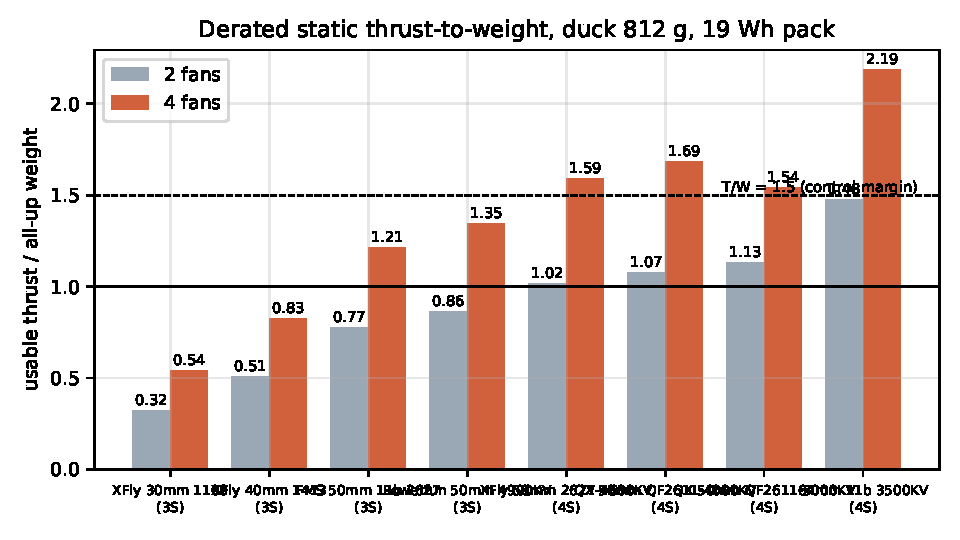
\includegraphics[width=0.7\linewidth]{figures/flight_tw_trade.pdf}
\caption{Usable thrust over weight, two and four fans.}
\end{figure}
Two 50\,mm fans do not lift the duck with margin (best \flTwoFanTW) and two fixed fans control roll
only. \textbf{Four fans}; the 30 and 40\,mm classes cannot hover.

\subsection{Fan variant and pack: the effect of sag}
\begin{table}[h]\centering\small
\caption{Same 50\,mm fan family on a 4S \fpPackMah\,mAh pack at mid charge, 45\,A limit. Left block:
seller thrust derated to 80\,\%; right block: taken at face value.}
\setlength{\tabcolsep}{4pt}
\begin{tabular}{llrrrrrrrr}
\toprule
 & & \multicolumn{4}{c}{derated} & \multicolumn{4}{c}{as listed}\\
fan & seller row & T/W & $V_b$ & $i$ [A] & hover [A] & T/W & $V_b$ & $i$ [A] & hover [A]\\
\midrule
\tabinput duck_flight_variant_table.tex
\bottomrule
\end{tabular}
\end{table}
The 4000\,KV unit that looks best at its listed 16.2\,V reaches only 1.21 on the sagging pack; the
5000\,KV unit, held at its 45\,A rating by the ESC limit, reaches \fpPackTW. \textbf{Choice: QX-Motor
QF2611-5000KV}, also the only family found in both rotation directions.

\begin{figure}[h]\centering
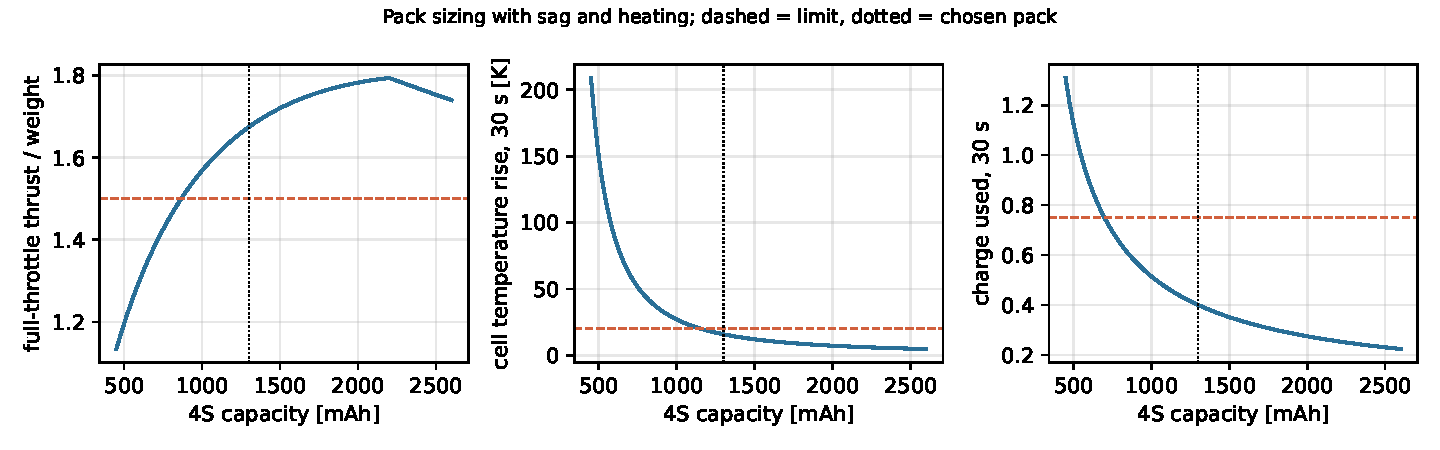
\includegraphics[width=0.7\linewidth]{figures/flight_pack_opt.pdf}
\caption{Pack constraints against capacity.}
\end{figure}
\begin{table}[h]\centering\small
\caption{Mass budget.}
\begin{tabular}{lr}
\toprule item & mass [g]\\ \midrule
\tabinput duck_flight_budget_table.tex
\bottomrule
\end{tabular}
\end{table}
The smallest commercial pack meeting all three constraints is \textbf{4S \fpPackMah\,mAh}
(\fpPackG\,g): thrust-to-weight \fpPackTW{} at \fpPackVfull\,V, hover at \fpPackUhover\,\% throttle,
\fpPackHoverA\,A (\fpPackC\,C), \fpPackDT\,K of heating and \fpPackSoc\,\% of charge in 30\,s, and
\fpPackHoverS\,s of hover to 20\,\%. Larger packs add little thrust margin (1.66 at 2200\,mAh).
\textbf{The design has not followed this result yet.} The pack was chosen as 1300\,mAh for an earlier, lighter
frame, and the bay, the mass budget (all-up \flAllUpG\,g, thrust-to-weight \flTW) and every simulation below still
carry it. With frame v8.1 the 1300\,mAh pack meets the thrust and charge constraints but heats by 20.7\,K in
30\,s against the 20\,K limit; it meets all three for a hover of 29\,s. A 1500\,mAh pack adds 25\,g and needs
its dimensions checked against the bay.
All-up mass is \flAllUpG\,g. Over a duck mass of 750--1000\,g and 68--100\,\% of listed thrust,
thrust-to-weight spans \flTwLow--\flTwHigh.
\begin{figure}[h]\centering
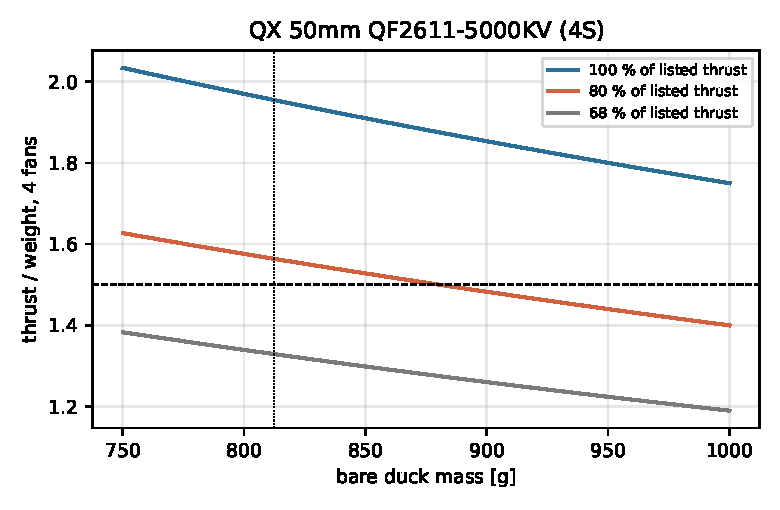
\includegraphics[width=0.7\linewidth]{figures/flight_tw_sensitivity.pdf}
\caption{Thrust-to-weight against the unweighed duck mass and the thrust derating.}
\end{figure}

\subsection{Identification pipeline on synthetic data}
\begin{table}[h]\centering\small
\caption{Recovery of a known plant from simulated bench logs with sensor noise (5\,g, 0.3\,\% rpm,
0.4\,A, 20\,mV). \emph{Synthetic}: this validates the procedure, not the fan.}
\begin{tabular}{llrrrlrr}
\toprule
parameter & unit & prior & truth & fit & 95\,\% interval & prior err [\%] & fit err [\%]\\
\midrule
\tabinput duck_flight_sysid_table.tex
\bottomrule
\end{tabular}
\end{table}
\begin{figure}[h]\centering
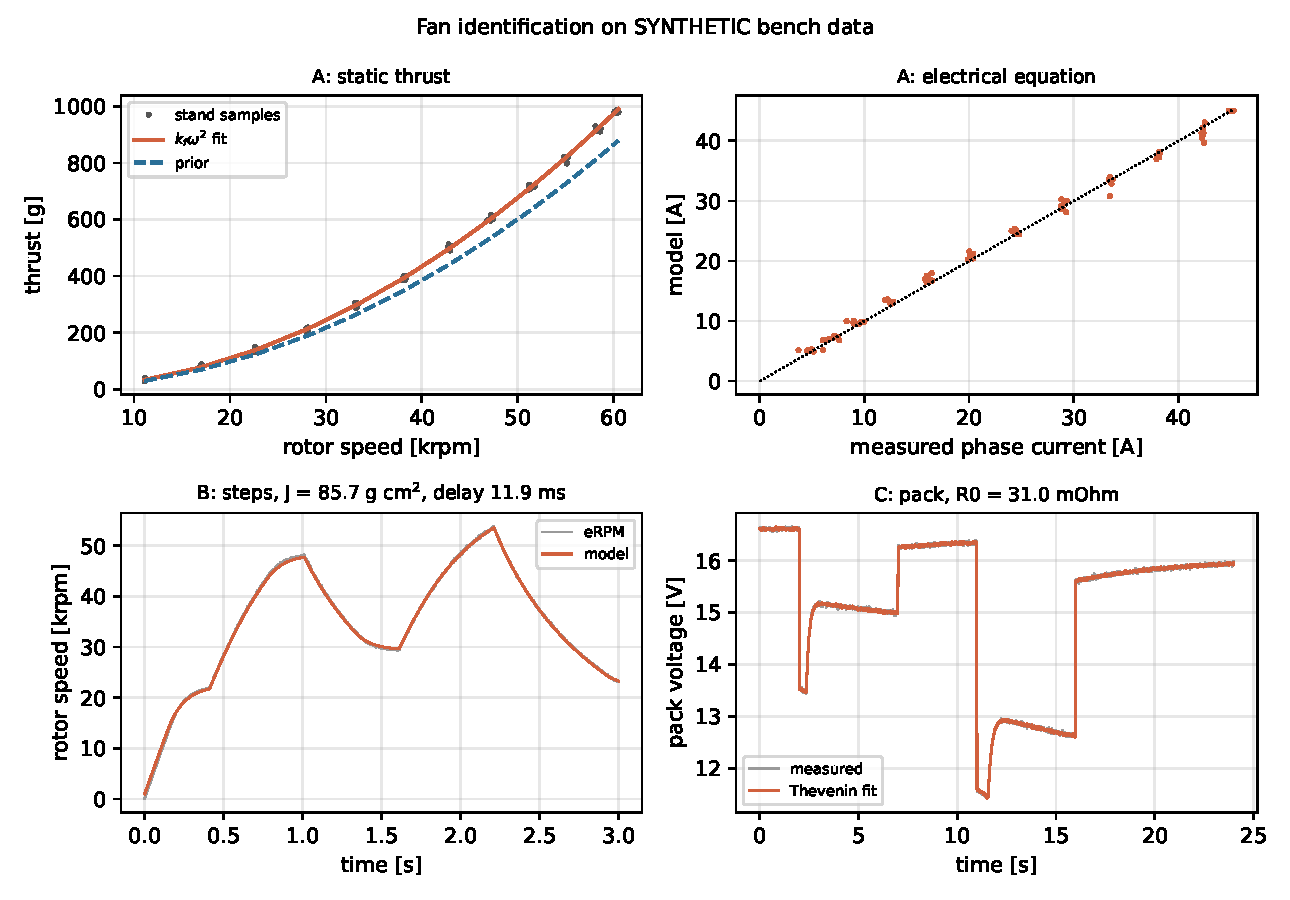
\includegraphics[width=0.7\linewidth]{figures/fan_sysid.pdf}
\caption{Fits of the three identification stages (synthetic data).}
\end{figure}
Thrust coefficient is recovered to \frSidKfErr\,\% (prior \frSidKfPrior\,\%), rotor inertia to
\frSidJErr\,\%, delay to \frSidDelayErr\,\%, pack resistance to \frSidRzeroErr\,\%. Winding resistance
is poorly conditioned from the static sweep alone (\frSidRErr\,\%; it trades against $K_e$) and
should be measured directly. Commanding the model's hover throttle on the true plant gives
\frSidHoverPrior\,\% of weight with the prior and \frSidHoverFit\,\% after identification.

\subsection{Placement}
\begin{figure}[h]\centering
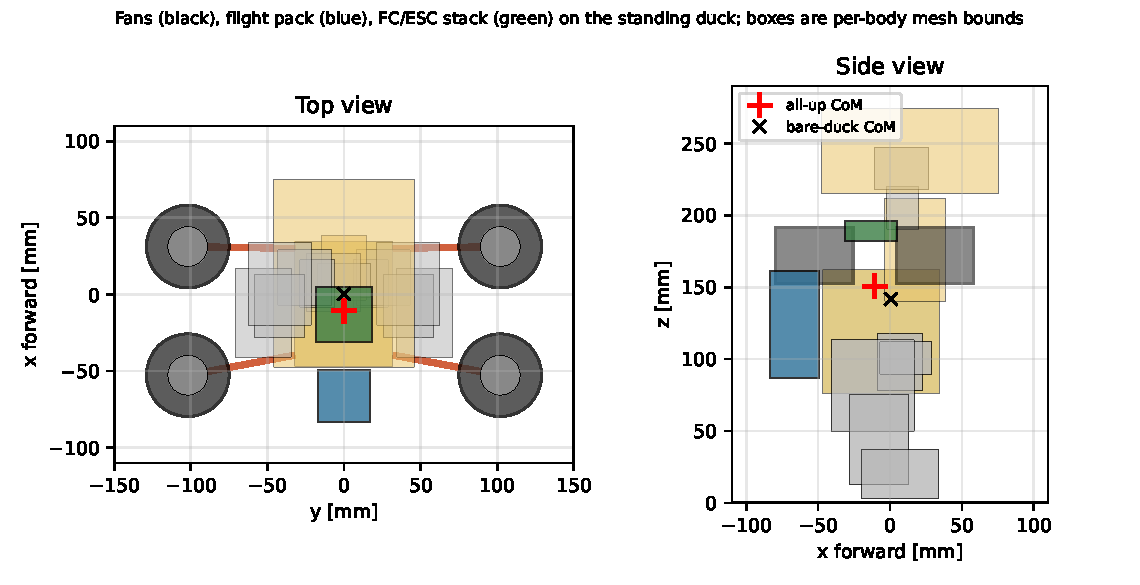
\includegraphics[width=0.7\linewidth]{figures/flight_layout.pdf}
\caption{Layout on the standing duck.}
\end{figure}
Fans are at $x=\flXc\pm42$\,mm, $y=\pm135$\,mm, mid-plane 220\,mm above the floor, i.e.\ above the trunk roof
(162\,mm) and outboard of the head's yaw sweep. The jets' inner edge clears the legs by \flClrStand\,mm and the
ducts clear the head by \flHeadClr\,mm in plan. Angular accelerations available are \flAccRoll,
\flAccPitch{} and \flAccYaw\,rad/s$^2$; sitting or folding the legs moves the centre of mass
\flSitDx/\flFoldDx\,mm, \flSitPct/\flFoldPct\,\% of pitch authority. Hip roll beyond
\flRollClearHi$^\circ$ outward puts a foot in a jet.

\subsection{Frame}\label{sec:v81}
\begin{figure}[h]\centering
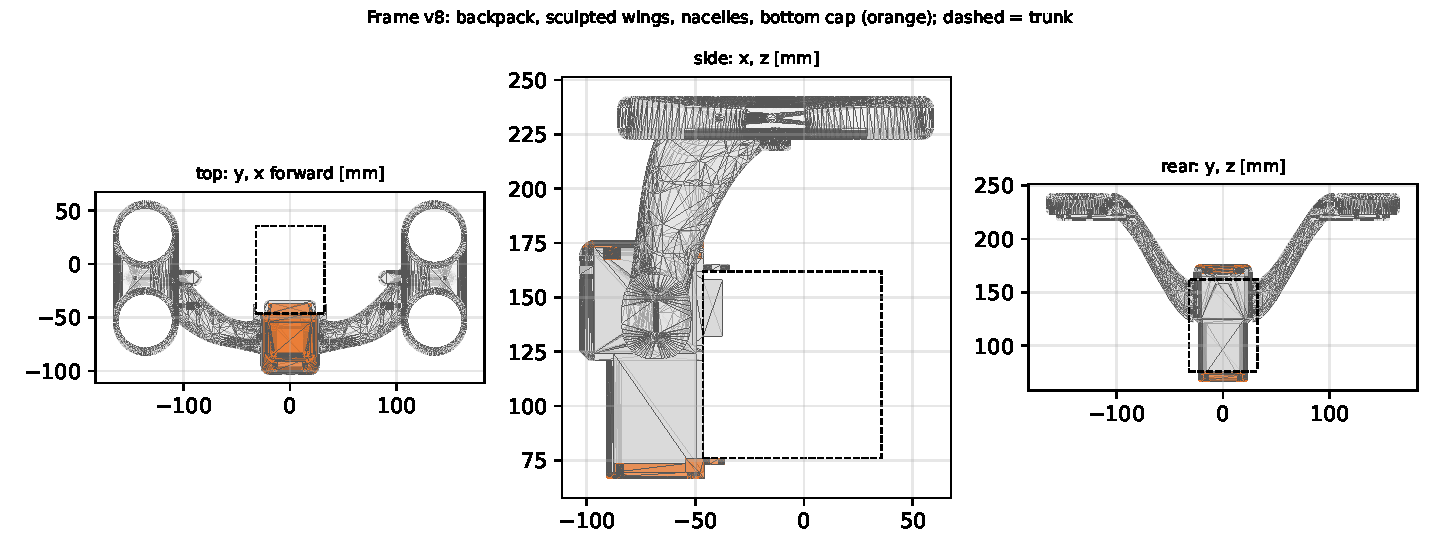
\includegraphics[width=0.7\linewidth]{figures/flight_frame.pdf}
\caption{Printed parts of frame v8.1: backpack with lid and bottom cap, two wings, two nacelles.}
\end{figure}
\textbf{Parts.} A backpack hooks over the rear edge of the trunk roof and is locked from below by a bottom cap;
it holds the pack upright and, in a wider head above $z=121$\,mm, the flight-controller stack under a removable
lid. One closed, sculpted wing per side (a loft through 13 superelliptic sections) runs from the head's side
wall to the inboard flank of a stadium-shaped nacelle that holds two fans; each fan slides in from below against
a shoulder, so thrust is carried in compression, and a ring with a grub screw keeps it in. Envelope
\frSpanY$\times$\frLenX\,mm; \frNParts{} printed parts, \frFramePLA\,g in PLA at 15\,\% infill with fasteners
(\frFramePLAB\,g at 25\,\%, \frFrameABS\,g in ABS). Earlier iterations, for the record: a collar frame (2.3\,mm
lift, $6^\circ$ tilt, 16\,Hz), spars across the roof (blocked \frClrHeadOld\,\% of head and neck poses), and
exposed trusses (stiff but rejected on appearance).

\textbf{Wing-to-nacelle joint.} A tongue under the nacelle takes two vertical M3 screws. Because nothing then
crossed the flank where the wing tip butts against the nacelle, two horizontal M3$\times$12 screws also pass
through the wing tip itself, $\pm12$\,mm about the tip's centre, into heat-set inserts in the nacelle's flank
(the web between the fans, $8.6$\,mm of material at the holes). Each head sits on $7$\,mm of wing material at the
bottom of a $6.2$\,mm channel that opens on the wing's top surface inboard of the tip. Each joint therefore has
four screws on two perpendicular axes, and no part was added. A version with a raised land on the nacelle and an
ear on each side of the wing tip also passed the checks below but added a visible flange and $9$\,g; it was
dropped.

\textbf{Stress and stiffness.} Table~\ref{tab:stress} lists all load cases at 15\,\% and 25\,\% infill
(\frStDofs\,k degrees of freedom, \frStMesh\,mm elements; core modulus \frStCoreE\,MPa and crush strength
\frStCoreS\,MPa at 15\,\%). At full thrust the fans move \frStDefl\,mm and tilt \frStTilt$^\circ$, the skin
stress is \frStVm\,MPa, and the lowest safety factor over all cases is \frStSfMin{} (\frStWorst; \frStSfMinB{} at
25\,\%). The first mode with the four fans as lumped masses is \frStMode\,Hz (\frStModeB\,Hz at 25\,\%), about
three times the attitude bandwidth: the margin is small, and 25\,\% infill buys little. \emph{The mesh is not
converged:} refining to \frStConvMesh\,mm (\frStConvDofs\,k degrees of freedom) changes the full-thrust
deflection by \frStConvDefl\,\% and the skin stress by \frStConvVm\,\% and gives a first mode of
\frStConvMode\,Hz, so the coarse values are conservative by about that much but no asymptote has been shown.
The new screw holes (3.4 and 6.2\,mm) are below the element size and the lid is not in the model.
\begin{table}[h]\centering\small
\caption{Frame v8.1, PLA: fan deflection [mm] and tilt [deg], skin von Mises and first principal stress [MPa],
core von Mises stress [MPa], largest principal strain [\%], and safety factors in the layer plane, across layers
and for core crushing.}\label{tab:stress}
\begin{tabular}{llrrrrrrrrr}\toprule
Infill & Load case & defl. & tilt & $\sigma_{\rm vM}$ & $\sigma_1$ & core & $\varepsilon$ & SF$_{xy}$ & SF$_z$ & SF$_{\rm c}$\\\midrule
\csname @@input\endcsname duck_flight_stress_table
\bottomrule\end{tabular}\end{table}
\begin{figure}[h]\centering
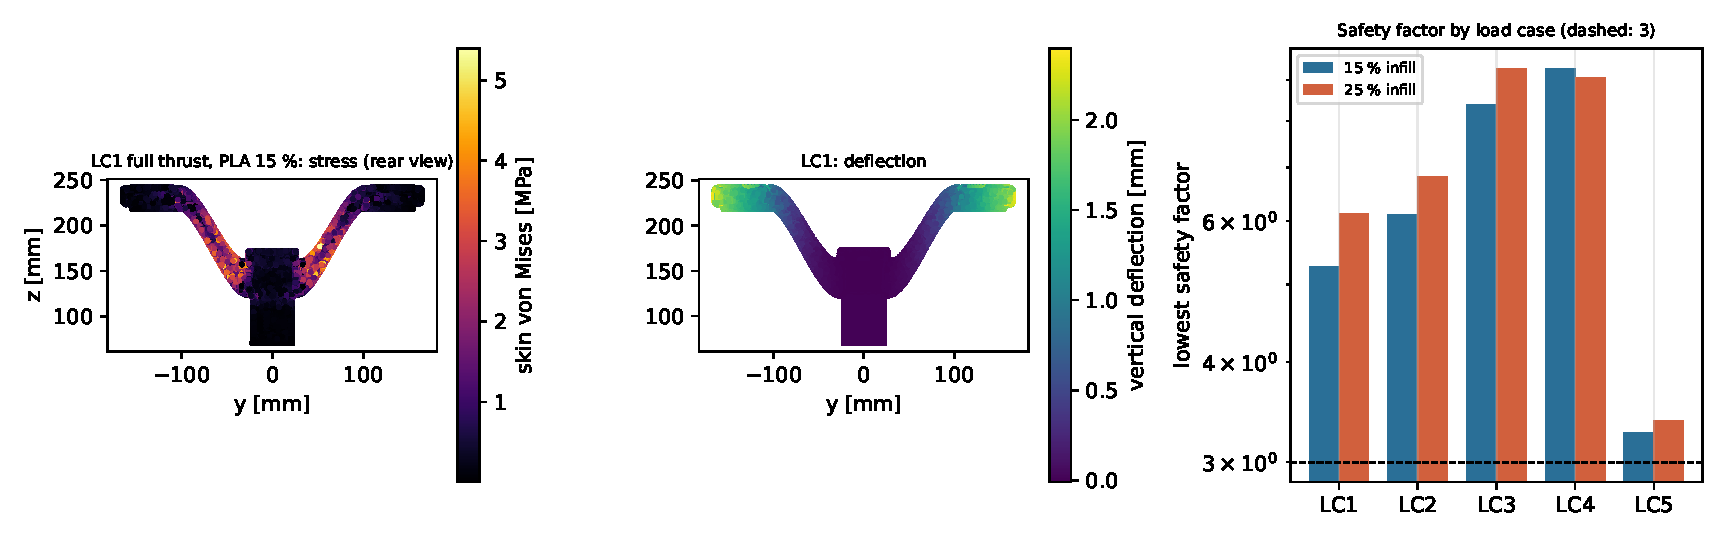
\includegraphics[width=0.7\linewidth]{figures/flight_stress.pdf}
\caption{Frame v8.1 at full thrust (LC1, 15\,\% infill): stress and deflection.}
\end{figure}

\textbf{Joint clearance.} With the frame's collision primitives and the four fans, \frClrHead\,\% of sampled
head and neck poses and \frClrLeg\,\% of leg poses are blocked (the spar frame: \frClrHeadOld\,\% and
\frClrLegOld\,\%); from the stand pose the left hip pitch is free from $-90^\circ$ to $+54^\circ$ and the head yaw
to $\pm85^\circ$.

\textbf{Tool access: definition.} For a screw with head position $\mathbf p$ and outward axis $\mathbf a$, a driver
shank is modelled as a cylinder of radius $r=2$\,mm (a 2.5\,mm hex key) leaving $\mathbf p$ along a direction
$\mathbf d$ with $\angle(\mathbf d,\mathbf a)\le 25^\circ$ (ball-end limit). The free length
$\ell(\mathbf d)=\min\{s>s_0 : \|\mathbf q-\mathbf p-s\mathbf d\|_\perp<r\}$ is taken over points $\mathbf q$ sampled on the
surfaces of the parts present at that assembly step ($4\times10^5$ area-weighted points per part, seed 0; the fans as
cylinders, the trunk as a box), ignoring the first $s_0=3$\,mm inside the counterbore, and is cut off at 120\,mm. A screw
passes if $\ell\ge 28$\,mm (an 8\,mm screw plus a 20\,mm tool) for some admissible $\mathbf d$. The check is a
point-sample test: it can miss an obstacle thinner than the sample spacing (about 0.3\,mm here), and it does not
model the hand or the long arm of the key.

\textbf{What the check found.} (i) In the version with ears, the rear ear's screw directly behind the wing tip had
$\ell=3.0$\,mm on its axis and $6.8$\,mm at $25^\circ$: the wing itself was in the way (moving it $14$\,mm aft
gave $\ell\ge120$\,mm). In the final version the channels through the wing tip are clear on their axes. (ii) The
electronics bay ($38\times39$\,mm) had been sized for a bare 36\,mm board; the chosen stack's ESC is
$45.6\times44$\,mm. Widening the whole backpack to $47\times48$\,mm raised the blocked leg poses from $23.3\,\%$ to
$27.8\,\%$ (left hip pitch free only to $+12^\circ$ instead of $+54^\circ$) and the walk--take-off--land baseline
no longer completed, so only the upper part of the backpack (above $z=121$\,mm, where the wing roots attach) was
widened. (iii) The stack then cannot pass up through the lower bay, so the head has a removable lid: the stack bolts
under the lid on the bench, the lid tucks a tab into the front wall and takes two screws into inserts in the head's
rear wall ($6.5$\,mm thick for that purpose). Table~\ref{tab:tool} and Fig.~\ref{fig:tool} give the final values.

\begin{table}[h]\centering
\caption{Free length for a driver at each screw of the final frame (left side; the right side mirrors). All pass on
the screw axis itself (tilt $0^\circ$); needed: 28\,mm.}\label{tab:tool}
\begin{tabular}{llr}\toprule
Screw & Driver comes from & Free length [mm]\\\midrule
Tongue, 2 per side & below the nacelle, between the fans & $\ge 120$\\
Through the wing tip, 2 per side & inboard, above the wing & $\ge 120$\\
Wing root, 2 per side & inside the head bay (open top) & 48\\
Lid, 2 & above & $\ge 120$\\
Bottom cap, 2 & below & $\ge 120$\\\bottomrule
\end{tabular}\end{table}

\begin{figure}[h]\centering
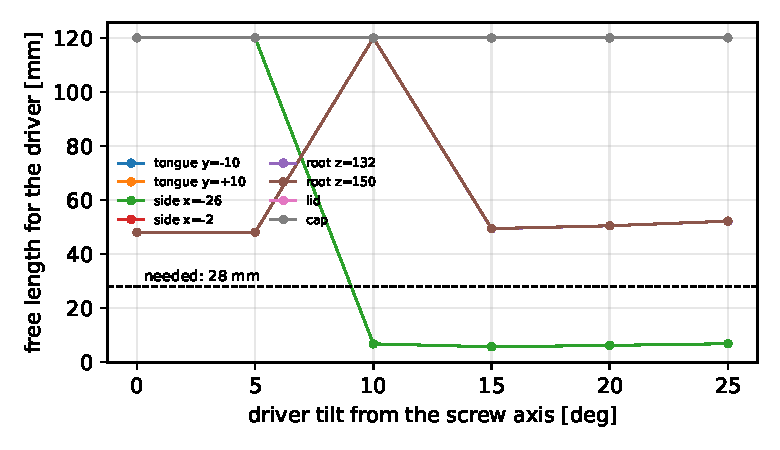
\includegraphics[width=0.7\linewidth]{figures/flight_tool_clearance.pdf}
\caption{Largest free length over azimuth against driver tilt, for each screw of the final frame.}\label{fig:tool}
\end{figure}

\textbf{Effect on the design.} Against frame v8 (ten parts, 248\,g, all-up 1603\,g, thrust-to-weight 1.56,
blocked poses $18.5\,\%$ and $23.3\,\%$) the changes of this subsection cost 25\,g and 0.02 of thrust-to-weight
and leave the free ranges of the leg joints unchanged. The Isaac Lab trainings queued before the change used the
v8 mass properties and must start from the new ones.

\textbf{Flight controller.} SpeedyBee F405~V4 with its 60\,A BLHeli\_S 4-in-1 ESC, hung under the lid; a three-wire
3.3\,V serial link (MSP) to the duck's computer, with arming and the kill switch kept on a radio receiver. Wiring,
firmware settings and open checks are in \texttt{docs/duck\_flight\_bom.md}. None of it has been bench-tested.

\subsection{MuJoCo: carrying the pack, and run to take-off}
With the fans off and a forward command for 6\,s over six servo-delay and supply variants, the bare
duck walks at \frCarryWalkBare\,m/s and runs at \frCarryRunBare\,m/s with no falls; with the \frPackG\,g of flight
hardware the deployed policies fall \frCarryWalkFalls{} (walk) and \frCarryRunFalls{} (run). On the ground the
fans therefore carry the hardware's weight and hold roll and pitch; the run policy then reaches \frRoRun\,m/s.
\begin{figure}[h]\centering
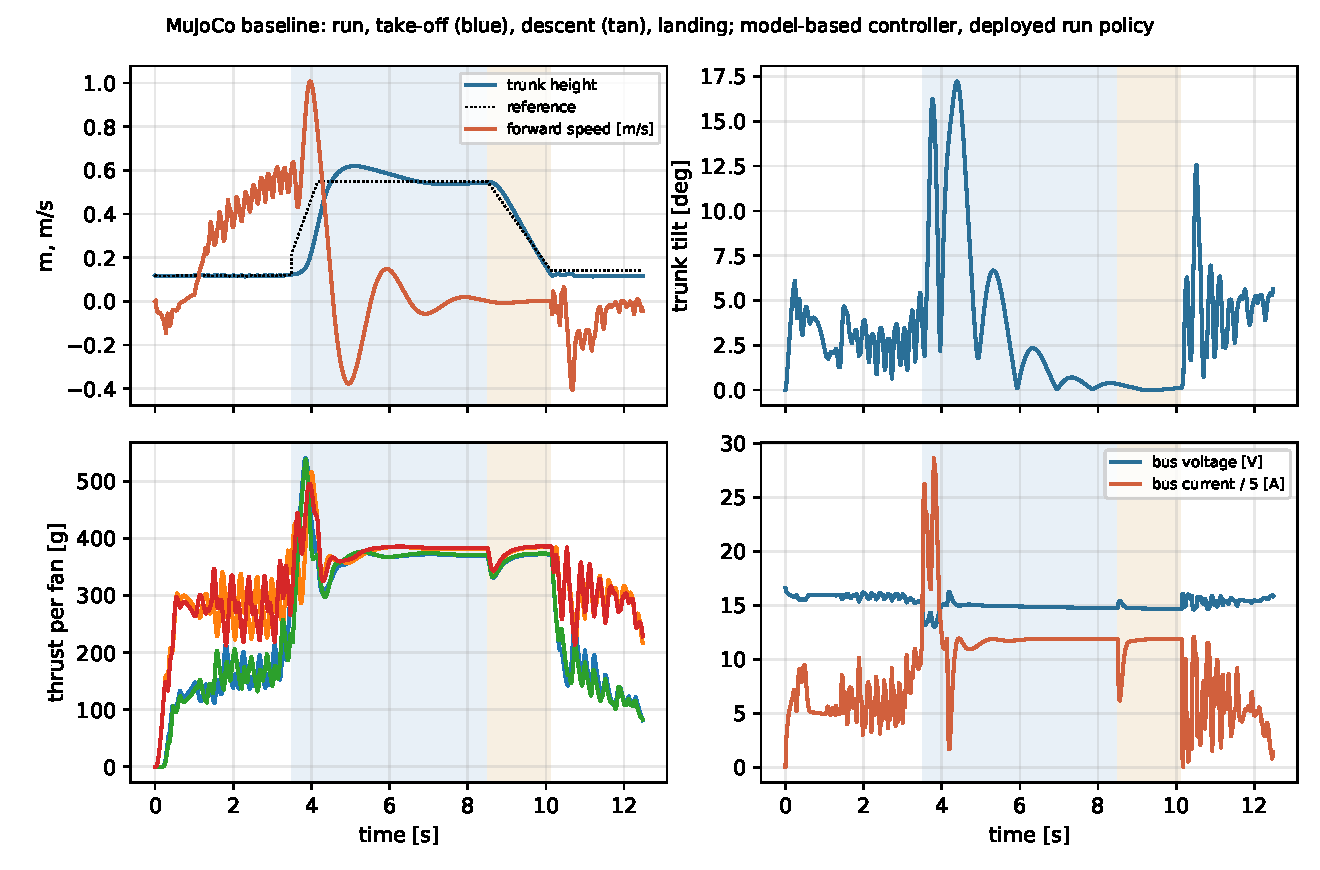
\includegraphics[width=0.7\linewidth]{figures/flight_rollout.pdf}
\caption{Thrust-assisted run, take-off, hover and landing (model-based controller, deployed run policy).}
\end{figure}
\begin{figure}[h]\centering
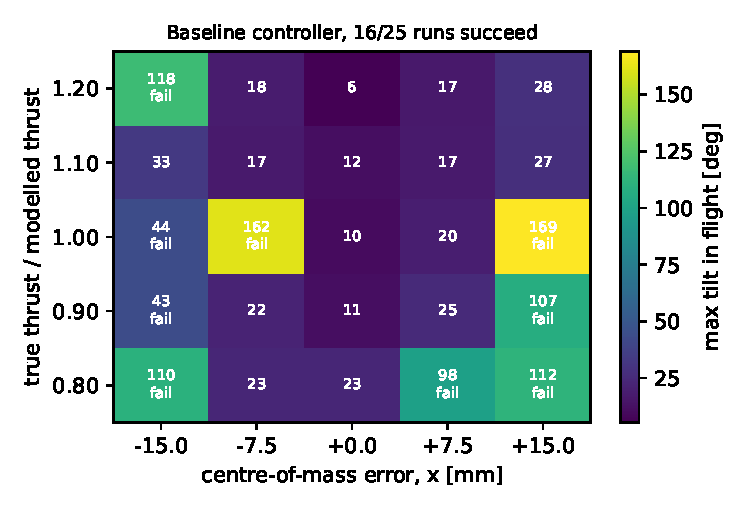
\includegraphics[width=0.7\linewidth]{figures/flight_rollout_robust.pdf}
\caption{Take-off from a stand (fans carrying \frRobAssist{} of the hardware's weight beforehand) with the true thrust
scaled and the controller's centre-of-mass belief shifted.}
\end{figure}
Nominal rollout (one deterministic run): lift-off at \frRoVlift\,m/s, maximum tilt \frRoTilt$^\circ$, hover height
error \frRoZerr\,mm and drift \frRoHoverV\,cm/s, hover at \frRoU\,\% throttle, \frRoI\,A and \frRoV\,V,
\frRoSoc\,\% of charge for the fan time, upright after landing. The tilt is close to the $35^\circ$ success limit:
the fore-aft fan spacing is only 84\,mm, so pitch authority is a third of roll authority (\flTauPitch{} against
\flTauRoll\,N\,m).

Against model error, with take-off from a stand and the fans carrying \frRobAssist{} of the hardware's weight
beforehand, \frRobOk{} of \frRobN{} runs succeed: \frRobThrustOk{} for thrust errors of $\pm20$\,\% alone,
\frRobComSmallOk{} with a $\pm7.5$\,mm centre-of-mass error, \frRobComBigOk{} at $\pm15$\,mm; the failures are
with the centre of mass believed too far aft, or at one $+10$\,\% thrust case. This experiment depends on the
ground assist: with none, the standing policy falls under the pack before take-off (0 of 25), with 0.5 only 8 of
25 succeed, and with the default 1.2 the nominal stand take-off flips in the air. The
walk--take-off--land--walk sequence, run for braked stops of 1.2 to 2.0\,s before take-off, took off, hovered
(error 11--13\,mm) and touched down upright in 5 of 5 runs, with a maximum tilt between $11^\circ$ and
$53^\circ$ (one run over the limit). The controller is therefore a baseline that works near its tuning point, not
a robust solution; the handover depends on the gait phase and on how much the fans carry.


\subsection{Learned flight policy (MuJoCo on a CPU): a negative result}
With the GPU machine unreachable, a flight policy was trained with PPO in MuJoCo on nine CPU cores, on the same fan
and pack model with its parameters redrawn every episode (thrust $\pm20$\,\%, per fan $\pm7$\,\%, rotor inertia
$\times0.7$--1.8, cell resistance $\times0.6$--1.6, command delay 5--20\,ms, centre of mass $\pm12$\,mm). The command
is a velocity in the heading frame, $(v_x, v_y, v_z, \dot\psi)$: the walk's command with a vertical component, so
take-off is a positive $v_z$ from the ground. Three findings.
\begin{itemize}
\item \textbf{From scratch it did not learn to fly.} After 3\,M steps the policy balanced on the ground with the fans
but crashed within 1.6\,s from 15 of 16 mid-air starts. Two errors were found on the way: body rates were read in the
trunk's inertial-axis frame instead of the body frame, and a narrow velocity kernel gave no gradient from standstill.
\item \textbf{The classical controller flies the same environment} at the same 50\,Hz, so the policy was retrained as
a residual on it: four fan corrections in mixer coordinates plus offsets on the ten leg joints, with a cost on
differential thrust so that a steady offset is cheaper to answer with the legs.
\item \textbf{The residual did not help.} After \frRlSteps\,M steps (\frRlMin\,min) and on the same 100 randomised
robots with random commands, the policy finishes \frRlPolOk{} episodes without a crash and the base controller alone
\frRlBaseOk. Horizontal velocity error is \frRlPolVxy\,m/s against \frRlBaseVxy\,m/s (worse), vertical
\frRlPolVz{} against \frRlBaseVz\,m/s. The legs move by up to \frRlLegDeg$^\circ$ with no measurable benefit.
On the nominal robot it follows a scripted sequence (take off, hover, forward, climb, sidestep, yaw, descend) without
crashing, tilting at most \frRlNomTilt$^\circ$.
\end{itemize}
\begin{figure}[h]\centering
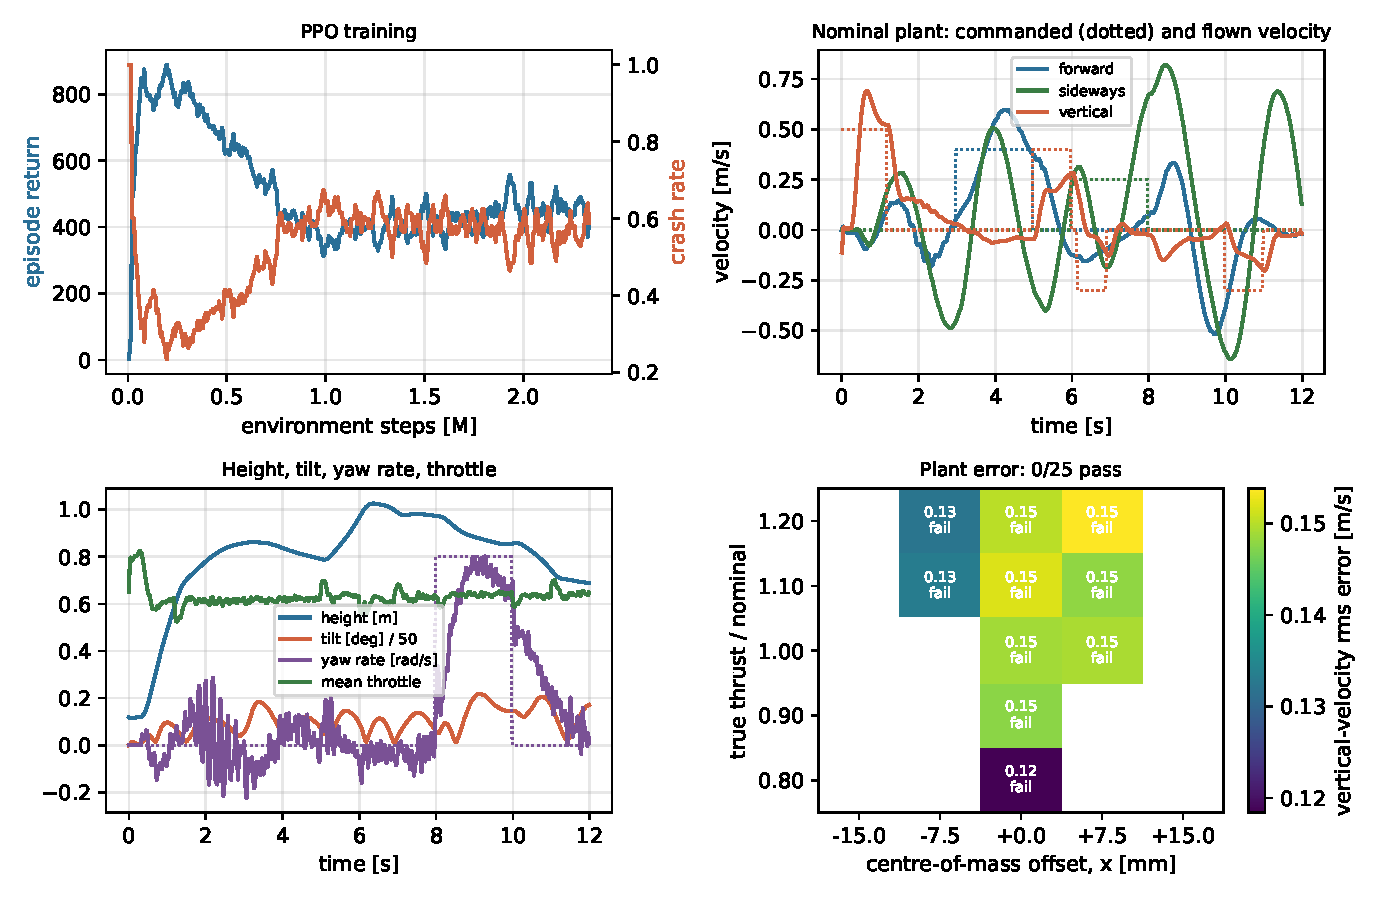
\includegraphics[width=0.7\linewidth]{figures/flight_rl_res_legs.pdf}
\caption{Residual policy: training curve, the nominal command sequence, and vertical-velocity error against plant error.}
\end{figure}
The limiting factor is the base controller, which under this randomisation survives 20 of 30 episodes at
$\pm5$\,mm of centre-of-mass error and 7 of 30 at $\pm12$\,mm; raising its trim gain made it unstable. Related work
(\texttt{docs/duck\_flight\_related\_work.md}) points to the remedies: one policy over legs and fans trained at GPU
scale, action history in the observation, and thrust-rate or body-rate commands.

\section{Implementation and Usage}\label{sec:use}
{\small
\begin{verbatim}
python scripts/tools/flight_design.py            # budget, layout, screening
.venv-cad/bin/python cad/flight/build_parts.py   # STEP/STL (run the pair twice)
python scripts/tools/flight_power.py             # pack and KV choice with sag
.venv-cad/bin/python cad/flight/fea_stress.py    # stress, stiffness, modes (20 min)
.venv-cad/bin/python scripts/tools/flight_tool_clearance.py  # tool access
python scripts/tools/flight_model.py             # flight_pack.json, MuJoCo scenes
~/.venvs/microduck_live/bin/python scripts/tools/flight_rollout.py
python scripts/tools/fan_sysid.py [--stand a.csv --step b.csv --pack c.csv]
python scripts/tools/flight_clearance_final.py   # blocked joint poses (10 min)
.venv-cad/bin/python cad/flight/make_drawings.py # 2D drawings
python scripts/tools/flight_print_orient.py      # print-oriented STL
python scripts/tools/flight_print_bambu.py       # Bambu Studio projects
python scripts/tools/flight_assembly_export.py   # web guide geometry
python scripts/tools/flight_assembly_page.py     # web assembly guide
python scripts/tools/flight_report.py && make -C docs
scripts/train_flight_chain.sh                    # GPU machine: Isaac Lab training
\end{verbatim}}
Constants: \texttt{scripts/tools/flight\_config.py}. Model: \texttt{microduck\_rl/flight/fan\_model.py}
(numpy or torch; the two agree to 0.002\,rad/s). Isaac Lab terms:
\texttt{microduck\_rl/mdp/flight.py}; tasks \texttt{Microduck-WalkPack-}, \texttt{-RunPack-} and
\texttt{-Takeoff-Flat-HD1910-AllColl}. Bill of materials: \texttt{docs/duck\_flight\_bom.md};
drawings: \texttt{cad/flight/drawings/}. Hardware path: one 4S pack, a 4-in-1 ESC held to 45\,A per fan (see the bill of materials for how)
and a flight controller logging rotor speed, current and voltage; the duck's computer sends
throttles or attitude setpoints. Rendering: \texttt{scripts/tools/isaacsim\_replay\_flight.py}
replays the recorded trajectory in Isaac Sim with a smoke emitter per fan.

\section{Limitations}\label{sec:lim}
\begin{itemize}
\item \textbf{No hardware data.} Every fan number is a seller row; $R$, $I_0$, $J$, $\kappa$ and the
pack resistance are assumed. The identification has only been run on synthetic logs.
\item \textbf{No working learned flight policy.} The CPU-trained policy does not beat the classical controller, and neither is robust to centre-of-mass error.
\item \textbf{Not trained:} the Isaac Lab tasks (walk and run with the pack, and the full walk--take-off--land
cycle) pass their smoke tests on the GPU machine and the fan model there matches the numpy one, but no training has
run to completion. The task's robot asset has no flight-hardware meshes yet. No Isaac Sim render exists; the
rollout videos made so far are MuJoCo previews.
\item \textbf{Nothing printed.} Print orientations, insert pockets, the lid's tab and the screw lengths are untested.
The stress analysis is not mesh-converged (\frStConvDefl\,\% in deflection on refinement), treats bolted joints as
bonded and does not resolve the screw holes. The first mode (\frStMode\,Hz) is close to the control bandwidth.
\item The duck is unweighed; a 1\,kg duck with fans at 68\,\% of listing has thrust-to-weight \flTwLow.
\item The frame is fitted to the official model's shell and to a 54.0\,mm shroud from one seller
page; the real shell and shroud may differ. The electronics bay is sized from one listing of the stack, and the
slot for its USB port is an estimate.
\item No aerodynamics beyond momentum theory: inlet distortion beside the trunk, jets on the legs and
ground effect are one factor of 0.95.
\item The baseline controller uses the simulator's true state, fails for a centre of mass believed
7.5\,mm or more too far aft in some cases, and depends on the ground-assist level and the gait phase at handover.
\item Hover lasts under a minute and one fan failing is not survivable.
\item Taobao was not searched (browser not connected); vendor links are to other shops.
\end{itemize}

\begin{thebibliography}{10}
\bibitem{leishman} J. G. Leishman, \emph{Principles of Helicopter Aerodynamics}, 2nd ed., Cambridge Univ. Press, 2006.
\bibitem{pereira} J. L. Pereira, ``Hover and wind-tunnel testing of shrouded rotors for improved micro air vehicle design,'' Ph.D. thesis, Univ. of Maryland, 2008.
\bibitem{mahony} R. Mahony, V. Kumar, P. Corke, ``Multirotor aerial vehicles: modeling, estimation, and control of quadrotor,'' \emph{IEEE Robotics \& Automation Magazine}, 19(3), 2012.
\bibitem{agilicious} P. Foehn et al., ``Agilicious: open-source and open-hardware agile quadrotor for vision-based flight,'' \emph{Science Robotics}, 7(67), 2022.
\bibitem{neurobem} L. Bauersfeld, E. Kaufmann, P. Foehn, S. Sun, D. Scaramuzza, ``NeuroBEM: hybrid aerodynamic quadrotor model,'' \emph{Robotics: Science and Systems}, 2021.
\bibitem{swift} E. Kaufmann et al., ``Champion-level drone racing using deep reinforcement learning,'' \emph{Nature}, 620, 2023.
\bibitem{ferede} R. Ferede, C. De Wagter, D. Izzo, G. C. H. E. de Croon, ``End-to-end reinforcement learning for time-optimal quadcopter flight,'' \emph{IEEE Int. Conf. on Robotics and Automation}, 2024.
\bibitem{gibson} L. J. Gibson, M. F. Ashby, \emph{Cellular Solids: Structure and Properties}, 2nd ed., Cambridge Univ. Press, 1997.
\bibitem{leo} K. Kim et al., ``A bipedal walking robot that can fly, slackline, and skateboard,'' \emph{Science Robotics}, 6(59), 2021.
\end{thebibliography}
\end{document}
